% !TeX TXS-program:compile = txs:///arara
% arara: lualatex: {shell: no, synctex: yes, interaction: batchmode}
% arara: pythontex: {rerun: modified} if found('pytxcode', 'PYTHONTEX#py')
% arara: lualatex: {shell: no, synctex: yes, interaction: batchmode} if found('pytxcode', 'PYTHONTEX#py')
% arara: lualatex: {shell: no, synctex: yes, interaction: batchmode} if found('log', '(undefined references|Please rerun|Rerun to get)')

\documentclass[a4paper,11pt]{article}
\usepackage[revgoku]{cp-base}
\graphicspath{{./graphics/}}
%variables
\donnees[classe={1\up*{ère} 2M2},matiere={[SPÉ.MATHS]},mois=Juin,annee=2022,typedoc=CHAP,numdoc=13]

%formatage
\author{Pierquet}
\title{\nomfichier}
\hypersetup{pdfauthor={Pierquet},pdftitle={\nomfichier},allbordercolors=white,pdfborder=0 0 0,pdfstartview=FitH}
%fancy
\lhead{\entete{\matiere}}
\chead{\entete{\lycee}}
\rhead{\entete{\classe{} - \mois{} \annee}}
\lfoot{\pied{\matiere}}
\cfoot{\logolycee{}}
\rfoot{\pied{\numeropagetot}}

\begin{document}

\pagestyle{fancy}

\part{CH13 - Fonction exponentielle - Exercices (Correction)}

\exonum{0}

\medskip

On utilise les propriétés algébriques de la fonction exponentielle :
\begin{enumerate}
	\item $\dfrac{\left(\e^3\right)^4 \times \e^3}{\e^4} = \dfrac{\e^{4 \times 3} \times \e^3}{\e^4} = \dfrac{\e^{12} \times \e^3}{\e^4} = \dfrac{\e^{15}}{\e^4}=\e^{15-4}=\e^{11}$.
	\item $\e^{x+4} \times \e^{4x} = \e^{x+4+4x}=\e^{5x+4}$.
	\item $\dfrac{1}{\e^{2-3x}} = \e^{-(2-3x)}= \e^{3x-2}$.
	\item $\e \times \dfrac{3\e^{5x}}{\left(\e^{x+1}\right)^3} = \e^1 \times \dfrac{3\e^{5x}}{\e^{3(x+1)}} = \dfrac{3\e^{1+5x}}{\e^{3x+3}} = 3\e^{1+5x-(3x+3)} = 3 \e^{2x-2}$.
\end{enumerate}

\medskip

\exonum{2}

\begin{enumerate}
	\item Pour tout réel $x$, on a :
	\begin{enumerate}
		\item $\e^x \left( \e^x + x \right) = \e^x \times \e^x + \e^x \times x = \e^{2x} + x\e^x$ .
		\item $\left( 1+\e^x \right)\left(1-\e^x\right) = 1 - \e^x + \e^x - \e^x \times \e^x = 1 - \e^{2x}$.
		\item $\left( \e^x + \e^{-x} \right)^2 =  \e^x \times \e^x + 2 \times \e^x \times \e^{-x} + \e^{-x} \times \e^{-x} = \e^{2x} + 2 \e^0 + \e^{-2x} = \e^{2x} + 2 + \e^{-2x}$.
		\item $\left( \e^{-2x}-\e^x \right)\left( \e^{-2x}+\e^x \right) = \e^{-2x} \times \e^{-2x} + \e^{-2x} \times \e^x - \e^x \times \e^{-2x} - \e^x \times \e^x = \e^{-4x} + \e^{-x} - \e^{-x} - \e^{2x} = \e^{-4x} - \e^{2x}$.
	\end{enumerate}
	\item 
	\begin{enumerate}
		\item $\dfrac{\e^x-1}{\e^x}=1-\e^{-x}$ car $\begin{dcases} \big(\e^x-1\big) \times 1 = \e^x-1 \\ \e^x \times \big( 1-\e^{-x} \big) = \e^x - \e^x \times \e^{-x} = \e^x - \e^0 = \e^x - 1 \end{dcases}$ pour tout réel $x$.
		\item $\dfrac{1}{\e^x+1}=\dfrac{\e^x-1}{\e^{2x}-1}$ car $\begin{dcases} 1 \times \big( \e^{2x}-1\big) = \e^{2x}-1 \\ \big( \e^x+1\big) \times \big(\e^x-1\big) = \e^x \times \e^x - \e^x + \e^x - 1 = \e^{2x} - 1  \end{dcases}$ pour tout réel $x$.
	\end{enumerate}
	\item On a $\e^{4x}+\e^x = \e^x \times \e^{3x} + \e^x = \e^x \times \big( \e^{3x} + 1\big)$ pour tout réel $x$.
	\item On a $3\e^x + \dfrac{2}{\e^x+3} = \dfrac{3\e^x \times \big(\e^x+3\big)+2}{\e^x+3} = \dfrac{3\e^{2x}+9\e^x+2}{\e^x+3}$ pour tout réel $x$. 
\end{enumerate}

\medskip

\exonum{2}

\smallskip

\begin{enumerate}
	\item On utilise les techniques classiques de résolution des équations, en \og rajoutant \fg{} la méthode \og $\e^{\ldots} = \e^{\ldots}$ \fg{} :
	\begin{enumerate}
		\item $\e^{x}=\e^{-2} \ssi x = -2$.
		\item $\e^{2x+1}=1 \ssi \e^{2x+1} = \e^0 \ssi 2x+1 = 0 \ssi x=-0,5$.
		\item $\e^{-x}-1=0 \ssi \e^{-x}=1 \ssi \e^{-x} = \e^0 \ssi -x = 0 \ssi x=0$.
		\item $10\e^{-x^2+2}+50=0 \ssi 10\e^{-x^2+2}=-50 \ssi \e^{-x^2+2} = -5$ ce qui est impossible !
		\item $(x-5)\e^{3x}=0$ est une équation produit nul :
		\begin{itemize}
			\item $x-5=0 \ssi x=5$ ;
			\item $\e^{3x}=0$ qui est impossible.
		\end{itemize}
		Ainsi $\mathscr{S}=\bigl\{ 5 \bigr\}$.
		\item $\left(x^2+2x+1\right)\left( 3\e^{x+2}-3 \right)=0$ est une équation produit nul :
		\begin{itemize}
			\item $x^2+2x+1=0$ : $\Delta = 0$ ce qui donne une racine, $x_0=-1$ ;
			\item $3\e^{x+2}-3=0 \ssi 3\e^{x+2}=3 \ssi \e^{x+2}=1=\e^0 \ssi x+2=0 \ssi x=-2$.
		\end{itemize}
		Ainsi $\mathscr{S}=\bigl\{ -2\,;\,-1 \bigr\}$.
	\end{enumerate}
	\pagebreak
	\item On utilise les techniques classiques de résolution des inéquations, en \og rajoutant \fg{} la méthode \og $\e^{\ldots} < \e^{\ldots}$ \fg{} :
	\begin{enumerate}
		\item $\e^{x} \pg \e^{-2} \ssi x \pg -2$ ce qui donne $\mathscr{S}=\intervFO{-2}{+\infty}$.
		\item $\e^{3x} < \e \ssi \e^{3x} < \e^1 \ssi 3x < 1 \ssi x < \tfrac{1}{3}$ ce qui donne $\mathscr{S}=\intervOF{-\infty}{\tfrac{1}{3}}$.
		\item $\e^{-2x-1} \pp 1 \ssi \e^{-2x-1} \pp \e^0 \ssi -2x-1 \pp 0 \ssi -2x \pp 1 \ssi x \pg -0,5$ ce qui donne $\mathscr{S}=\intervFO{-0,5}{+\infty}$.
		\item $\e^{-2x+1} -\e^{x-7} > 0 \ssi \e^{-2x+1} > \e^{x-7} \ssi -2x+1 > x-7 \ssi -3x > -8 \ssi x > \tfrac{8}{3}$ ce qui donne $\mathscr{S}=\intervOO{\tfrac{8}{3}}{+\infty}$.
		\item $\e^{x+4} \pg \dfrac{1}{\e^{3x}} \ssi \e^{x+4} \pg \e^{-3x} \ssi x+4 \pg -3x \ssi 4x \pg -4 \ssi x \pg -1$ ce qui donne $\mathscr{S}=\intervFO{-1}{+\infty}$.
		\item $(x-1)\e^x  > 0$ se présente bien sous la forme \textsf{ZPQ} pour lequel on cherche \og les $\oplus$ sans les zéros \fg{} :
		\begin{itemize}
			\item $x-1=0 \ssi x=1$ et $m=1 \oplus$ ;
			\item $\e^x$ est toujours strictement positif !
		\end{itemize}
		\begin{center}
			\begin{tikzpicture}
				\tkzTabInit{$x$/0.7,$(x-1)$/0.7,$\e^x$/0.7,expr/0.7}{$-\infty$,$1$,$+\infty$}
				\tkzTabLine{,-,z,+,}
				\tkzTabLine{,+,t,+,}
				\tkzTabLine{,-,z,+,}
			\end{tikzpicture}
		\end{center}
		Ainsi $\mathscr{S}=\intervOO{1}{+\infty}$.
	\end{enumerate}
	\item Les expressions suivantes sont présentées sous forme \textsf{Produit/Quotient}, on peut donc se lancer dans les tableaux de signes :
	\begin{enumerate}
		\item $(3x-1)\e^x$ :
		\begin{itemize}
			\item $3x-1=0 \ssi x=\tfrac13$ et $m=3 \oplus$ ;
			\item $\e^x$ est toujours strictement positif !
		\end{itemize}
		\begin{center}
			\begin{tikzpicture}
				\tkzTabInit{$x$/0.7,$(3x-1)$/0.7,$\e^x$/0.7,expr/0.7}{$-\infty$,$\tfrac13$,$+\infty$}
				\tkzTabLine{,-,z,+,}
				\tkzTabLine{,+,t,+,}
				\tkzTabLine{,-,z,+,}
			\end{tikzpicture}
		\end{center}
		\item $\dfrac{6x-12}{\e^{3x+1}}$ :
		\begin{itemize}
			\item $6x-12=0 \ssi x=2$ et $m=6 \oplus$ ;
			\item $\e^{3x+1}$ est toujours strictement positif !
		\end{itemize}
		\begin{center}
			\begin{tikzpicture}
				\tkzTabInit{$x$/0.7,$(6x-12)$/0.7,$\e^{3x+1}$/0.7,expr/0.7}{$-\infty$,$2$,$+\infty$}
				\tkzTabLine{,-,z,+,}
				\tkzTabLine{,+,t,+,}
				\tkzTabLine{,-,z,+,}
			\end{tikzpicture}
		\end{center}
		\item $(-24x^2+20x-4)\e^{x-2}$ :
		\begin{itemize}
			\item $-24x^2+20x-4=0$ : $\Delta=16$ ce qui donne deux racines, $x_1=\tfrac12$ et $x_2=\tfrac13$, avec de plus $a=-24 \ominus$ ;
			\item $\e^{x-2}$ est toujours strictement positif !
		\end{itemize}
		\begin{center}
			\begin{tikzpicture}
				\tkzTabInit[lgt=4]{$x$/0.7,$\big(-24x^2+20x-4\big)$/0.7,$\e^{x-2}$/0.7,expr/0.7}{$-\infty$,$\tfrac13$,$\tfrac12$,$+\infty$}
				\tkzTabLine{,-,z,+,z,-,}
				\tkzTabLine{,+,t,+,t,+,}
				\tkzTabLine{,-,z,+,z,-,}
			\end{tikzpicture}
		\end{center}
		\item $\dfrac{\e^x-1}{(x+3)^2}$ :
		\begin{itemize}
			\item $\e^x-1 \pg 0 \ssi \e^ \pg 1 \ssi \e^x \pg \e^0 \ssi x \pg 0$ ;
			\item $(x+3)^2$ est le carré d'un expression s'annulant en $x=-3$.
		\end{itemize}
		\begin{center}
			\begin{tikzpicture}[double distance=2]
				\tkzTabInit[]{$x$/0.7,$\e^x-1$/0.7,$(x+3)^2$/0.7,expr/0.7}{$-\infty$,$-3$,$0$,$+\infty$}
				\tkzTabLine{,-,t,-,z,+,}
				\tkzTabLine{,+,z,+,t,+,}
				\tkzTabLine{,-,d,-,z,+,}
			\end{tikzpicture}
		\end{center}
	\end{enumerate}
\end{enumerate}

\medskip

\exonum{2}


\begin{enumerate}
	\item $f(x)=\e^x-x^2$ se dérive (sur $\R$) comme une somme :
	
	\hspace{0.5cm}$f'(x)=\e^x - 2x$.
	\item $g(x)=10\e^x+\dfrac1x$ se dérive (sur $\R^*$) comme une somme :
	
	\hspace{0.5cm}$g'(x)=10 \times \e^x - \dfrac{1}{x^2} = 10\e^x - \dfrac{1}{x^2}$.
	\item $h(x)=\e^{3x}+\e^{-5x+4}$ se dérive (sur $\R$) comme une somme :
	
	\hspace{0.5cm}$h'(x)=3\e^{3x}+\left(-5\e^{-5x+4}\right)=3\e^{3x}-5\e^{-5x+4}$.
	\item $i(x)=(x+3)\e^x$ se dérive (sur $\R$) comme un produit:
	
	\hspace{0.5cm}$i'(x)=1 \times \e^x + \e^x \times (x+3) = \e^x (1+x+3)=\e^x(x+4)$.
	\item $j(x)=10\e^{-x}+7\e^{2x}$ se dérive (sur $\R$) comme une somme :
	
	\hspace{0.5cm}$j'(x)=10 \times \left(-\e^{-x}\right) + 7 \times \left(2\e^{2x}\right) = -10\e^{-x}+14\e^{2x}$.
	\item $k(x)=\dfrac{x}{\e^x}$ se dérive (sur $\R$) comme un quotient :
	
	\hspace{0.5cm}$k'(x)=\dfrac{1 \times \e^x - \e^x \times x}{\left(\e^x\right)^2} = \dfrac{\e^x(1-x)}{\e^{2x}}=\dfrac{1-x}{\e^x}$.
	\item $l(x)=\dfrac{\e^x-1}{\e^x+1}$  se dérive (sur $\R$) comme un quotient :
	
	\hspace{0.5cm}$l'(x)=\dfrac{\e^x\big(\e^x+1\big)-\e^x\big(\e^x-1\big)}{\big(\e^x+1\big)^2}=\dfrac{\e^x \big( \e^x+1-(\e^x-1)\big)}{\big(\e^x+1\big)^2} = \dfrac{2\e^x}{\big(\e^x+1\big)^2}$.
	\item $m(x)=(25x+40)\e^{-0,2x}$ se dérive (sur $\R$) comme un produit :
	
	\hspace{0.5cm}$m'(x)=25 \times \e^{-0,2x} + \left(-0,2 \times \e^{-0,2x}\right) \times (25x+40) = \e^{-0,2x} \times \big( 25-0,2(25x+40) \big) = (-5x+17)\e^{-0,2x}$.
	\item $o(x)=\big(x^2-3x+1\big)\e^x$ se dérive (sur $\R$) comme un produit :
	
	\hspace{0.5cm}$o'(x)=(2x-3)\e^x+\e^x(x^2-3x+1)=\e^x(2x-3+x^2-3x+1)=(x^2-x-2)\e^x$.
\end{enumerate}

\medskip

\exonum{2}

\smallskip

\begin{enumerate}
	\item 
	\begin{enumerate}
		\item La fonction $f$ est dérivable sur $\R$ et, pour tout $x$, on a $f'(x)=\e^x$.
		\item On a $f'(x)=\e^x >0$ sur $\R$, donc $f$ est strictement croissante sur $\R$.
	\end{enumerate}
	\item 
	\begin{enumerate}
		\item La fonction $g$ est dérivable sur $\R$ et, pour tout réel $x$, on a $g'(x)=10 \times \left(-2 \times \e^{-2x+6} \right) = -20 \e^{-2x+6}$.
		\item On a $g'(x)=-20 \e^{-2x+6} <0$ sur $\R$, donc $g$ est strictement décroissante sur $\R$.
	\end{enumerate}
	\item 
	\begin{enumerate}
		\item La fonction $h$ est dérivable (produit) sur $\R$ et, pour tout réel $x$ :
		
		\hspace{0.5cm}$h'(x)=2\times \e^x + \e^x \times (2x+3)=\e^x \times (2+2x+3) = (2x+5)\e^x$.
		\item On voit que $h'(x)$ se présente sous forme d'un produit :
		\begin{itemize}
			\item $2x+5=0 \ssi x=-2,5$ avec $m=2 \oplus$ ;
			\item $\e^x$ est strictement positif !
		\end{itemize}
		\begin{center}
			\begin{tikzpicture}
				\tkzTabInit[]{$x$/0.7,$(2x-5)$/0.7,$\e^x$/0.7,$f'(x)$/0.7}{$-\infty$,${-2,5}$,$+\infty$}
				\tkzTabLine{,-,z,+,}
				\tkzTabLine{,+,t,+,}
				\tkzTabLine{,-,z,+,}
			\end{tikzpicture}
		\end{center}
		\item On peut donc en déduire les variations de $h$ sur $\R$ :
		\begin{center}
			\begin{tikzpicture}
				\tkzTabInit[]{$x$/0.7,$f'(x)$/0.7,$f$/1.4}{$-\infty$,${-2,5}$,$+\infty$}
				\tkzTabLine{,-,z,+,}
				\tkzTabVar{+/,-/${f(-2,5)}$,+/}
			\end{tikzpicture}
		
			Avec $f(-2,5) = (2 \times (-2,5) + 3) \e^{-2,5} = -2\e^{-2,5} \approx -0,164$ au millième.
		\end{center}
	\end{enumerate}
\end{enumerate}

\medskip

\exonum{3}

\begin{enumerate}
	\item La fonction $f$ est dérivable (produit) sur $\R$ et, pour tout réel $x$, on a :
	
	\hspace{0.5cm}$f'(x)=5 \times \e^{-0,2x} + \left(-0,2 \times \e^{-0,2x}\right) \times (5x+7) = \e^{-0,2x} \times \big( 5 -0,2(5x+7) \big) = (5-x-1,4)\e^{-0,2x}=(-x+3,6)\e^{-0,2x}$
	\item 
	\begin{enumerate}
		\item On voit que $f'(x)$ se présente sous forme d'un produit :
		\begin{itemize}
			\item $-x+3,6=0 \ssi x=3,6$ avec $m=-1 \ominus$ ;
			\item $\e^{-0,2x}$ est strictement positif !
		\end{itemize}
		\begin{center}
			\begin{tikzpicture}
				\tkzTabInit[]{$x$/0.7,${(-x+3,6)}$/0.7,$\e^{-0,2x}$/0.7,$f'(x)$/0.7}{$-\infty$,${3,6}$,$+\infty$}
				\tkzTabLine{,+,z,-,}
				\tkzTabLine{,+,t,+,}
				\tkzTabLine{,+,z,-,}
			\end{tikzpicture}
		\end{center}
		\item On peut donc en déduire les variations de $f$ sur $\R$ :
		\begin{center}
			\begin{tikzpicture}
				\tkzTabInit[]{$x$/0.7,$f'(x)$/0.7,$f$/1.4}{$-\infty$,${3,6}$,$+\infty$}
				\tkzTabLine{,+,z,-,}
				\tkzTabVar{-/,+/${f(3,6)}$,-/}
			\end{tikzpicture}
			
			Avec $f(3,6) = (5 \times 3,6 + 7) \e^{-0,2 \times 3,6} = 25\e^{-0,72} \approx 12,169$ au millième.
		\end{center}
	\end{enumerate}	
	\item Une équation de $\mathscr{T}_0$ est donnée par $y=f'(0) \times (x-0) + f(0)$ :
	\begin{itemize}
		\item $f(0)=(5 \times 0+7) \e^{-0,2 \times 0} = 7\e^0=7$ ;
		\item $f'(0)=(-0+3,6) \e^{-0,2 \times 0} = 3,6\e^0 = 3,6$.
	\end{itemize}
	Ainsi $\mathscr{T}_0$ : $y=3,6 \times x + 7 = 3,6x+7$.
\end{enumerate}

\begin{center}
	\tunits{2}{0.5}
	\tdefgrille{0}{7}{0.5}{0.25}{0}{14}{2}{1}
	\begin{tikzpicture}[x=\xunit cm,y=\yunit cm]
		\tgrilles ; \tgrillep ;
		\axestikz* ; \axextikz{0,0.5,...,6.5} ; \axeytikz{0,2,...,12} ;
		\draw[red,line width=1.25pt,samples=250,domain=0:7] plot (\x,{(5*\x+7)*exp(-0.2*\x)}) ;
		\draw[blue,line width=1.25pt,<->,>=stealth'] (1.6,12.169) -- (5.6,12.169) ;
		\filldraw[blue] (3.6,12.169) circle[radius=2.5pt] ;
		\draw[red] (7,10.357) node[below left] {\Large $\mathscr{C}_f$} ;
		\draw[ForestGreen,samples=2,domain=0:1.944,line width=1.25pt] plot (\x,{3.6*\x+7}) ;
		\draw[ForestGreen] (1.144,13.84) node[below right] {\Large $\mathscr{T}_0$} ;
	\end{tikzpicture}
\end{center}

\medskip

\exonum{3}

\begin{enumerate}
	\item Le résultat réalisé par la fabrication et la vente de $7$ centaines de litres de produit est donné par $R(7)$ dizaine de milliers d'euros. Or $R(7)=(5 \times 7 - 30) \e^{-0,25 \times 7} = 5\e^{-1,75} \approx 0,86887$, donc le résultat est d'environ \num{8689}\,€. 
	\item Pour la fabrication et la vente de $400$ litres de produit, on calcule $R(4)=(5 \times 4 - 30) \e^{-0,25 \times 4} = -10\e^{-1} \approx -3,6790$, qui est négatif et donc qui correspond bien à un déficit.
	\item On a, sachant qu'une exponentielle est strictement positive :
	
	\hspace{0.5cm}$R(x) \pg 0 \ssi (5x-30)\e^{-0,25x} \ssi 5x-30 \pg 0 \ssi 5x \pg 30 \ssi x \pg 6$.
	
	Dans le contexte de l'exercice, on obtient le fait que l'entreprise réalise un bénéfice à partir de 600 ($6 \times 100$) litres de produit. 
	\item 
	\begin{enumerate}
		\item La fonction $R$ est dérivable (produit) sur $\intervFF{2}{20}$ et, pour tout réel $x \in \intervFF{2}{20}$, on a :
		
		\hspace{0.5cm}$R'(x)=5 \times \e^{-0,25x} + \left(-0,25 \times \e^{-0,25x}\right) \times (5x-30) = \e^{-0,25x} \times \big( 5 -0,25(5x-30) \big) = (5-1,25x+7,5)\e^{-0,25x}$
		
		\hspace{0.5cm}$\phantom{R'(x)} = (-1,25x+12,5)\e^{-0,25x}$.
		\item On voit que $R'(x)$ se présente sous forme d'un produit :
		\begin{itemize}
			\item $-1,25x+12,5=0 \ssi -1,25x=-12,5 \ssi x= 10$ avec $m=-1,25 \ominus$ ;
			\item $\e^{-0,25x}$ est strictement positif !
		\end{itemize}
		\begin{center}
			\begin{tikzpicture}
				\tkzTabInit[lgt=4,deltacl=0.7]{$x$/0.7,${(-1,25x+12,5)}$/0.7,$\e^{-0,25x}$/0.7,$R'(x)$/0.7,$R$/1.4}{$2$,${10}$,$20$}
				\tkzTabLine{,+,z,-,}
				\tkzTabLine{,+,t,+,}
				\tkzTabLine{,+,z,-,}
				\tkzTabVar{-/$R(2)$,+/$R(10)$,-/$R(20)$}
			\end{tikzpicture}
		\end{center}
		
		Avec $R(2) \approx -12,1306$ ; $R(10) \approx 1,6416$ et $R(20) \approx 0,4716$ au dix-millième.
		\item La quantité de produit que l'entreprise doit produire et vendre pour réaliser le résultat maximal est de \num{1000} ($10 \times 100$).
	\end{enumerate}
\end{enumerate}

\end{document}